%
\documentclass[a4paper]{article}


\usepackage{color}              %Farben, f.r \definecolor{}
\usepackage{amssymb}            %Mathematische Symbole
\usepackage{amsthm}             %Besseres \newtheorem
\usepackage{amsmath}           %Mathematische Umgebungen
\usepackage{mathtools}          %\xRightarrow, etc
\usepackage{mathrsfs}           %enthaelt \mathscr
\usepackage[matrix,arrow,curve]{xy}     %Diagramme
\usepackage{graphicx}
\usepackage{enumerate}          % in-place numerations def.
\usepackage{fullpage}

\newcommand{\RR}{\mathbb{R}}
\newcommand{\ZZ}{\mathbb{Z}}

%% Dokument Beginn %%%%%%%%%%%%%%%%%%%%%%%%%%%%%%%%%%%%%%%%%%%%%%%%%%%%%%%%
\begin{document}
\pagestyle{empty}
\begin{center}
	{\Large\bf Graph coloring}\\
	{\large\bf Unit-distance-avoiding colorings of $\RR^2$}\\
	\line(1,0){330}
\end{center}

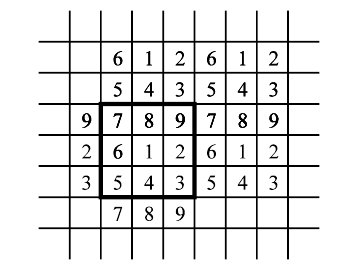
\includegraphics[scale=0.4]{mf8.png}

Naive $9$-coloring.

\bigskip

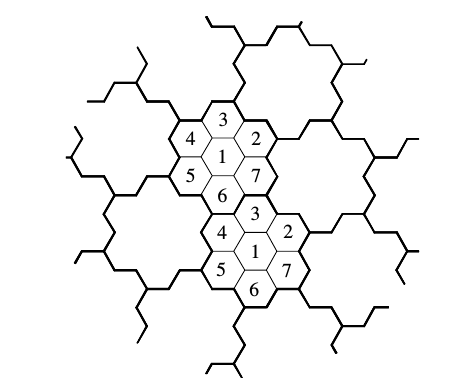
\includegraphics[scale=0.5]{mf5.png}  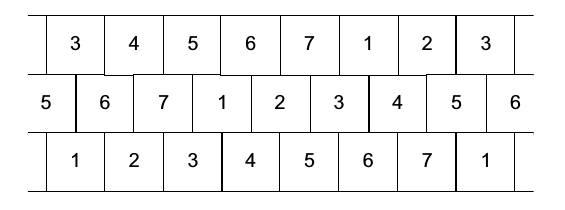
\includegraphics[scale=0.5]{mf9.png}

Colorings with $7$ colors.

\bigskip

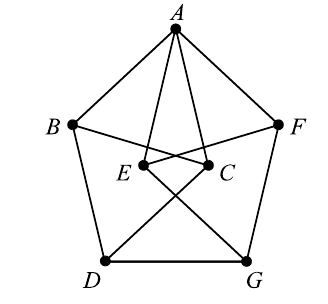
\includegraphics[scale=0.4]{mf6.png} 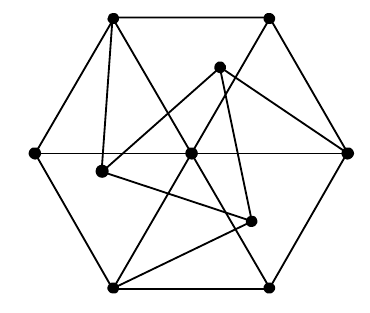
\includegraphics[scale=0.4]{mf7.png}

Moser graph and Golomb graph, unit distance graphs in $\RR^2$ with $\chi=4$.

\end{document}




